\section{Algorithm modification}\label{ps}

This section will outline some important  problems of current implementation and proposed solutions.


\subsection{Research motivation}

% There were experiments of GLL-based CFPQ algorithm implementation carried out on real graphs and compared with the Meerkat library\footnote{Meerkat.Graph library repository: \url{https://github.com/YaccConstructor/Meerkat}, accessed: 05/05/2022}. This library bases on parser combinators and also supports queries with context-free constraints. It also uses the Neo4j graph base as its graph repository.

There were experiments of GLL-based CFPQ algorithm implementation carried out on real graphs.
The experiment analysis showed that the algorithm demonstrated a good performance in most cases. It means that it is the right way in solving the problem of searching for paths in a graph with context-free constraints.

However, sometimes in the single source scenario an unexpected deterioration in the behavior of the resulting solution was revealed. Since the cause of performance problems remained unclear, as part of this work, it was decided to repeat experiments on a wider set of queries.
These experiments of the extended GLL algorithm showed that queries for some start vertex sets take an abnormally long time to complete compared to other queries of the same type. 

To sum up, despite of the efficiency showed by the algorithm, the behavioral problems call into a question its applicability in practice in the form in which it exists.

% The solution was profiled with Java Flight Recorder (JFR). The results showed that the largest amount of CPU time is spent in the main class method \texttt{Neo4jGraphInput --- nextSymbols}. This method is used to map the current input to a grammar terminal. It takes a vertex and returns a list of labels (symbols) on the outgoing  edges. At the same time, in order to obtain these labels, it is necessary to reach out to the Neo4j database. The Native Java API provides a convenient way to do this: to get an iterator over the set of outgoing edges using the \texttt{getRelationships.iterator()} method.
% However, in the current implementation, almost all CPU time is spent on calculations within the database.

\subsection{Problems and its solution}

This subsection describes the changes made to the algorithm implementation to improve its performance and to eliminate the identified problems.

First of all, the solution was profiled with Java Flight Recorder (JFR). The results showed that the largest amount of CPU time is spent in the main class method \texttt{Neo4jGraphInput --- nextSymbols}. This method is used to map the current input to a grammar terminal. It takes a vertex and returns a list of labels (symbols) on the outgoing  edges. At the same time, in order to obtain these labels, it is necessary to reach out to the Neo4j database. The Native Java API provides a convenient way to do this: to get an iterator over the set of outgoing edges using the \texttt{getRelationships.iterator()} method.
However, in the current implementation, almost all CPU time is spent on calculations within the database.

It should be noted that after the input matching with the terminal, it is possible that not all labels will be used in the further execution of the algorithm. Saving all the data leads to a huge overhead (up to a heap overflow) in case when degree of the vertex is very big, and most of the labels are discarded after matching.
Thus, it is necessary to optimize the transfer of labels from the database to further processing. The following solution was proposed.

A common and reasonable solution to this problem is using the Stream API. Stream in Java is a sequence of elements supporting sequential and parallel aggregate operations. In other words, it is not a data store, but an interface to the source, from where elements are taken only when they are needed. One scenario for using threads as the return type of a method is as follows. In the called method, one must specify the processing of objects using one or more intermediate operations, and in the calling method, the final operation. The \texttt{nextSymbols} method has been rewritten to accommodate this scenario for all input types. Now the data source is the Neo4j database, the intermediate operation is filtering edges by labels, and the final operation is getting labels from the stream returned by the \texttt{nextSymbols} method. Thus, in this method, stream processing of data was provided.

The modified algorithm was tested and re-profiled. The profiling results confirmed that the changes made to the \texttt{nextSymbols} method were correct and, thus, the problem of the algorithm's slowing was eliminated. Moreover, it will be demonstrated in Experimental Study section that the optimizations generally affected the speed of the algorithm in a positive direction.

\subsection{Functionality extension}
This section describes the changes that have been made to the algorithm for solving the reachability CFPQ problem.

Extended GLL algorithm returns SPPF. It contains all derivations trees for all paths which satisfy to language constraints. So there is provided a natural solution for the all paths CFPQ problem. But in practice, the restrictions on processor resources are very significant, while restoring the paths themselves is not always required. Often it is enough to obtain only information about its existence. Accordingly, there was added a switch that allows one to not to create SPPF in case when only reachability information. SPPF is needed only for paths reconstruction, so if one wants to get only reachable pairs, SPPF construction can be omitted, which leads to performance improvements and memory consumption decreasing.

\begin{figure}[ht]
    \centering
    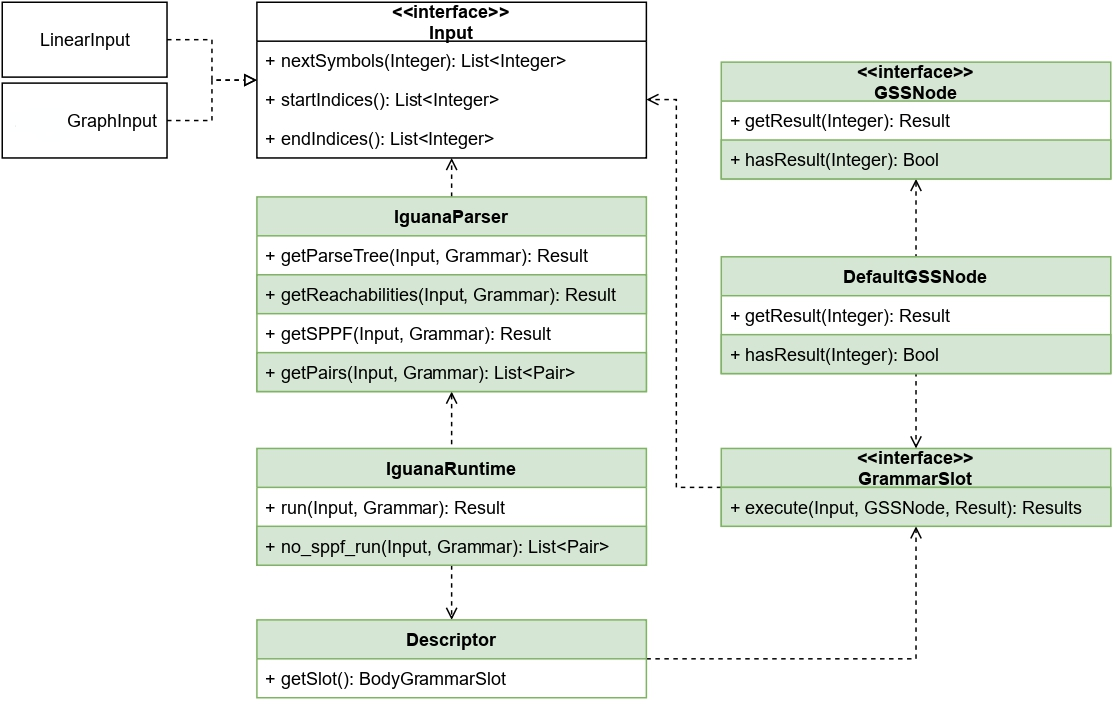
\includegraphics[width=0.95\textwidth]{figures/sppf_arch.jpg}
    \caption{Architecture of the solution}
    \label{fig:solution_architecture}
\end{figure}

The main parts of the solution are presented in figure~\ref{fig:solution_architecture}. To handle the scenario when SPPF construction is omitted almost all architecture elements were changed. The green color in this diagram marks the classes and methods that have been changed at this stage of the work. \texttt{Iguana Runtime} takes an \texttt{Input} and a context-free \texttt{Grammar} to produce the \texttt{Result}. The  \texttt{Result} is a key entity which should or should not contain SPPF information. \texttt{Input} abstracts a data structure with the ability to get the next symbols for the given position. One example of \texttt{Input} is \texttt{Graph}, in which the position is a vertex, and the next symbols are the labels of its outgoing edges. There was provided to use different forms of graph representation. Communication with the database is done using the Neo4j Native Java API. The way to create a database was changed. Now an embedded database is used. It means that it runs inside of the application and it is not used as an external service as it was earlier. Worth noting, the architecture is extensible, and one can provide their own implementation of \texttt{Graph} to enable context-free path querying for a new graph storage.